\section{Integration and Test Facility (ITF)}
\label{sec:fdsp-tc-itf}

%%%%%%%%%%%%%%%%%%%%%%%%%%%%
\subsection{Introduction}
\label{sec:fdsp-tc-itf-intro}

The components of the DUNE detectors will be manufactured in many numerous different countries and locations. For many of the parts it is reasonable to ship the components to the logistics warehouse and then receive the equipment underground where it can be installed. However the  cold electronics and the photon detectors are tightly coupled to the APA. The wires and filters on the APA form part of the electronics circuit and the photon supports and cabling are built into the APA. The work to integrate the CE and PD into the APA is large and the risk of damaging the components is significant so it is planned to integrate the components as early as possible and then thoroughly test the complete assembly. In order to avoid having to create integration testing facilities at each factory one central facility will be established in South Dakota near the SURF site  (within 1 hour drive). In this Integration Test Facility (ITF) the APA, CE and PD modules will arrive, undergo initial tests, be integrated together, undergo a set of warm tests, and then 10\% of the complete assemblies will be cold tested. As the fabrication of the APA assemblies must start 2 years before the completion of the detector installation in order to have enough time to fabricate all the APA the ITF needs to also be operational on the same timescale. The specifications for the ITF are summarized in Table \ref{tab:tcps-itf-spec}.

\begin{dunetable}
[ITF Specifications]
{cc}
{tab:tcps-itf-spec}
{Summary of the high level specifications for the ITF. The building requirements are covered separately in a separate section.}
Parameter & Specification \\ \toprowrule
Cleanroom & The ITF cleanroom shall meet ISO-8 standard per ISO-14644 \\ \colhline
Filtered Lights & <520 nm for long exposure and <400 for exposures less than 2 weeks \\ 
\end{dunetable}

\href{https://lbne2-docdb.fnal.gov/cgi-bin/private/RetrieveFile?docid=8348&filename=UVblockerTests.pdf&version=1 }{UV light filter Study}

%%%%%%%%%%%%%%%%%%%%%%%%%%%%
\subsection{APA-CE-PD integration}
\label{sec:fdsp-tc-itf-integ}
\begin{dunefigure}[ITF Cleanroom Layout]{fig:fdsp-tc-itf-clean}
{Conceptual layout of the cleanroom for the APA-CE-PD integration and testing.}
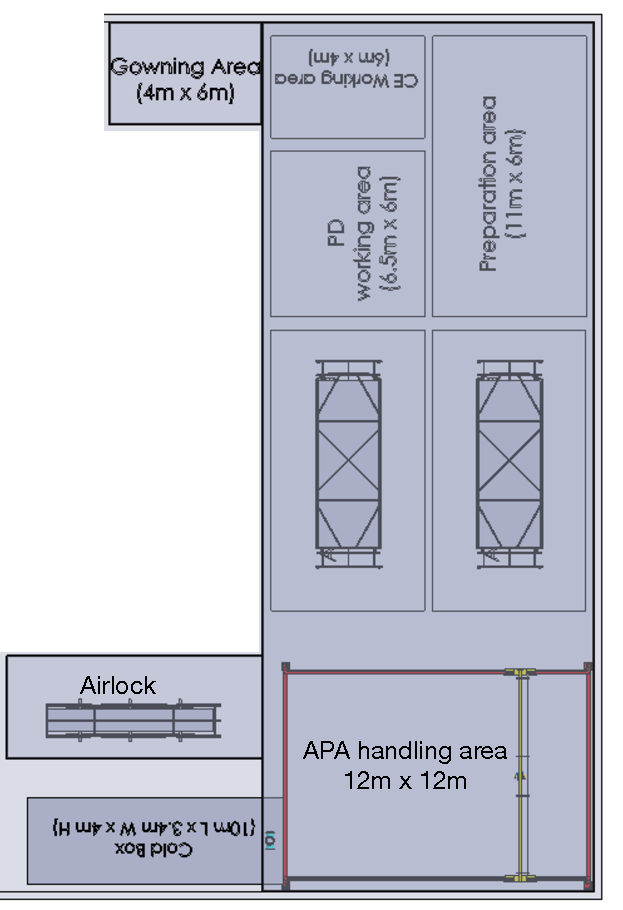
\includegraphics[width=0.8\textwidth]{itf-clean}
\end{dunefigure}

Most the work in the ITF must be done in a cleanroom environment to protect the components from dust and unfiltered light. The cleanliness requirement for the detector components is ISO-8 which corresponds to filtered air with clean lab coats, clean shoes, and hair nets. To protect the photon detector's TPB coating the lights need to be filtered to remove frequencies below 520nm. One possible layout of the cleanroom is shown in Figure \ref{fig:fdsp-tc-itf-clean} . Materials enter the ITF cleanroom through the materials airlock. This area needs to be sufficiently large accommodate the APA transport boxes and allow workers to move around the box to remove the dirty shipping layer and prepare for transport into the cleanroom. Other materials will also through the airlock but they will need much less space. The CE and PD equipment will be moved to the PD work area and preparation area where the components are unpacked and tested. The tests performed are described in detail in the Quality Management section below. The APA will enter cleanroom through the airlock and initially go to the APA handling area where an overhead workstation or gantry crane will be available. The APA will then be removed from the transport box and mounted to a process cart which can rotate the APA horizontally. The process cart will be pushed to one of the two APA integrations areas and then prepared for the installation of the CE and PD. During the integration process the APA will be held horizontal and the PDs will be inserted into the sides while the cold electronic boxes are mounted to the end of the APA. After the component integration the system will be tested and then either moved back to the handling area and boxed for return to the logistics center for storage or inserted into the cold box for further cryogenic testing. 

All the detector  components will arrive at the ITF either from the logistics facility or directly from the factories. Sufficient space will be needed inside the ITF but outside the cleanroom to store several weeks of material and a few boxes of the integrated APA boxes. Additionally a changing room is needed for the workers to change into clean cloths and shoes. The capacity of the changing room should be sufficient for roughly 20 workers in the cleanroom. 

%%%%%%%%%%%%%%%%%%%%%%%%%%%%
\subsection{Quality Management}
\label{sec:fdsp-tc-itf-qaqc}
Extensive testing of the detector components will be performed inside the IFT facility as the APA-PD-CE integration takes place. These tests form a vital part of the quality control process for DUNE. Details of the tests for each of the components are described below.

\subsubsection{Cold Electronics}

\subsubsection{APA}

\subsubsection{Photon Detectors}

%%%%%%%%%%%%%%%%%%%%%%%%%%%%
\subsection{Building Requirements and Infrastructure}
\label{sec:fdsp-tc-itf-req}
The ITF building requirements are summarized in DocDb 11500.
\cite{bib:docdb11500} 

The building to be used as the ITF facility has not been identified at present. In order to assist in identify or designing the ITF building a set of requirements were drafted. The requirements document defines the spaces needed for the integration work while not specifying the final layout of the cleanroom. This will allow the configuration of the cleanroom spaces to be adapted to possible building footprints as candidate buildings are identified. As the building has not been identified yet the cleanroom layout shown in Figure \ref{fig:fdsp-tc-itf-clean} should be taken as a concept and the final layout may change to adapt to the footprint of the final building. The building requirements document\cite{docdb-11500}  defines the minimum spaces for all the operations inside the ITF cleanroom, it defines the space needed for the cold box and the related cryogenic system, it provides guidance for the space needed for material storage outside the cleanroom, and it established the power and other general requirements the building must fulfill. Some requirements depend on the location of the building and the facilities available in the area. For example office space for 20 scientists working in the ITF will be needed in the area but  this would not need to be in the ITF building if local options are available. Some local machining facilities also fall into this category. 

%%%%%%%%%%%%%%%%%%%%%%%%%%%%
\subsection{Safety}
\label{sec:fdsp-tc-itf-safety}


%%%%%%%%%%%%%%%%%%%%%%%%%%%%
\subsection{Cost, Schedule and Risk Analysis}
\label{sec:fdsp-tc-itf-cost}

\fixme{use templates from cost-risk-sched.tex file. Anne}
